\documentclass[english]{beamer}

\usepackage{babel}
\usepackage{fontspec}
\usepackage{microtype}

\usepackage{csquotes}

\usepackage{amssymb,amsmath}

\usepackage[
            backend=biber,
            style=numeric,
            isbn=false,
            doi=false
        ]{biblatex}

\addbibresource{sources.bib}

% Colors
\usepackage{xcolor}
\definecolor[named]{uboBlue}{cmyk}{1,.7,0,0}
\definecolor[named]{uboYellow}{cmyk}{0,.3,1,0}
\definecolor[named]{uboGrey}{cmyk}{0,0,.15,.55}

\usepackage{tikz}
\usetikzlibrary{calc,positioning}

% Theme
\usetheme{metropolis}
\usefonttheme{professionalfonts}

\metroset{block=fill}
\setbeamercolor{title}{fg=uboBlue}
\setbeamercolor{subtitle}{fg=normal text.fg}
\setbeamercolor{title separator}{fg=uboYellow}
\setbeamercolor{frametitle}{bg=black!20!uboBlue}
\setbeamercolor{itemize item}{fg=uboBlue}
\setbeamercolor{enumerate items}{fg=uboBlue}
\setbeamercolor{block title}{bg=uboYellow}

\title{An intro to multilinear maps and their attacks using the example of CLT13}
\author{Lukas Kempf}
\date{2021-12-10}

\newcommand*{\todo}[1]{\textcolor{red}{TODO:~#1}}

\usepackage{suffix}
\newcommand{\citeauthoryear}[1]{\citeauthor{#1} \citeyear{#1}}
\WithSuffix\newcommand\citeauthoryear*[1]{\citeauthor*{#1} \citeyear{#1}}

\newcommand*{\IN}{\mathbb{N}}
\newcommand*{\IZ}{\mathbb{Z}}

\usepackage{mathtools}
\DeclareMathOperator{\smod}{mod}
\DeclareMathOperator{\id}{id}
\DeclareMathOperator{\crt}{CRT}
\DeclareMathOperator{\diag}{diag}

\newcommand*{\crtp}[2][i]{\crt_{(p_{#1})}\left(\left[#2\right]\right)}

\usepackage{epsdice}
\newcommand*{\rand}{\mathrm{rand}}
\newcommand*{\rgets}{\xleftarrow{\rand}}

\newcommand*{\pubkey}{\mathrm{pubKey}}

\usepackage{hyperref}

\begin{document}
    \begin{frame}[plain]
        \titlepage
    \end{frame}
    \begin{frame}{Outline}
        \begin{itemize}
            \item Multilinear maps
            \item CLT13
            \item DH with CLT13
            \item Attacking CLT13
            \item State of multilinear maps
        \end{itemize}
    \end{frame}
    \begin{frame}{Diffie-Hellman key exchange}
        \setbeamercolor*{block title}{bg=uboGrey}
        Let $G$ be finite cyclic group with generator $g$.

        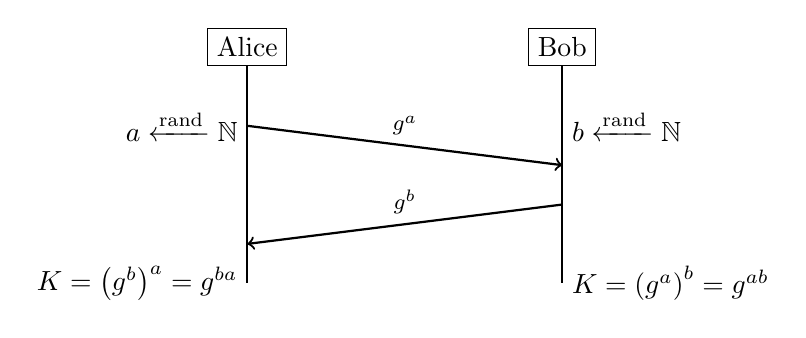
\begin{tikzpicture}
            % Alice
            \node[draw] (Alice) at (-2,0) {Alice};
            \draw[thick] (Alice) -- ++(0, -3);
              
            % Calculations of Alice
            \node[draw=none,fill=none,anchor=east] (asecret) at ($(Alice) + (0,-1)$) {$a \rgets \IN$};
            \node[draw=none,fill=none,anchor=east] (akey) at ($(Alice) + (0,-3)$) {$K = \left(g^b\right)^{a} = g^{ba}$};

            % Bob
            \node[draw] (Bob) at (2,0) {Bob};
            \draw[thick] (Bob) -- ++(0, -3);
             
            % Calculations of Bob
            \node[draw=none,fill=none,anchor=west] (bsecret) at ($(Bob) + (0,-1)$) {$b \rgets \IN$};
            \node[draw=none,fill=none,anchor=west] (bkey) at ($(Bob) + (0,-3)$) {$K = \left(g^a\right)^{b} = g^{ab}$};

            % Messages
            \draw[->,thick] ($(Alice)+(0,-1)$) -- ($(Bob)+(0,-1.5)$) node [pos=0.5,above,font=\footnotesize] {$g^a$};
            \draw[->,thick] ($(Bob)+(0,-2)$) -- ($(Alice)+(0,-2.5)$) node [pos=0.5,above,font=\footnotesize] {$g^b$};

        \end{tikzpicture}

        \pause
        $\Rightarrow$ Obtaining $g^{ab}$ from $g^a$ and $g^b$ this must be hard (computational assumption).

        \pause
        Alternative stronger assumption: Given $g^a$ and $g^b$ it must be hard to differentiate $g^{ab}$ from random (decisional assumption).
    \end{frame}
    \begin{frame}{Multilinear maps}
        \begin{definition}[Multilinear Map \citeauthoryear*{boneh2003applications}]
            A map $e: G_1^\kappa \rightarrow G_2$ is a \emph{$\kappa$-multilinear map} if it satisfies the following properties:
            \begin{enumerate}
                \item $G_1$ and $G_2$ are groups of the same prime order
                \item if $a_1,\dots ,a_\kappa \in \IZ$ and $x_1, \dots, x_\kappa \in G_1$ then
                    \begin{equation*}
                        e\left( x_1^{a_1}, \dots, x_n^{a_\kappa} \right) = e(x_1, \dots, x_n)^{a_1\dots a_\kappa}
                    \end{equation*}
                \item if $g \in G_1$ is a generator of $G_1$ then $e(g, \dots, g)$ is a generator of $G_2$.
            \end{enumerate}
        \end{definition}
    \end{frame}
    \begin{frame}{DH with multilinear maps}
        With multilinear maps: DH between multiple parties in one round.
        \pause

        Let $e: G_1^\kappa \rightarrow G_2$ be a $\kappa$-multilinear map and $g$ a generator of $G_1$.

        Each of the $\kappa+1$ parties chooses $a_i \rgets \IN$ and broadcasts $f_i = g^{a_i}$.

        \begin{multline*}
            e(f_2, \dots, f_{\kappa+1})^{a_1} = e(f_1, f_3, \dots, f_{\kappa+1})^{a_2} = \dots \\
            = e(f_1, \dots, f_\kappa)^{a_{\kappa+1}} = e(g, \dots, g)^{a_1 \cdots a_{\kappa+1}}
        \end{multline*}

        \pause
        Security assumption: Given $e, g, g^{a_1}, \dots, g^{a_{\kappa+1}} \in G_1$ it is hard to compute $e(g, \dots, g)^{a_1 \cdots a_{\kappa+1}} \in G_2$.
    \end{frame}
    \begin{frame}{How to construct such maps?}
        \blockquote[\citeauthoryear*{boneh2003applications}][]{The central open problem posed in this paper is the construction of cryptographic multilinear map generators when $\kappa > 2$.}
        \pause

        \blockquote[\citeauthoryear*{boneh2003applications}][]{We also give evidence that such maps might have to either come from outside the realm of algebraic geometry, or occur as \enquote{unnatural} computable maps arising from geometry.}
    \end{frame}
    \begin{frame}{Graded encoding schemes}
        Somewhat similar to homomorphic encodings.

        For every $r \in R$ and level $t \in \IN$ we have a set $S^{(r)}_t$ of possible encodings.

        Addition is possible: For $v_1 \in S^{(r_1)}_t$ and $v_2 \in S^{(r_2)}_t$ we have $v_1 + v_2 \in S^{(r_1 + r_2)}_t$.

        Multiplication is possible: For $v_1 \in S^{(r_1)}_{t_1}$ and $v_2 \in S^{(r_2)}_{t_2}$ we have $v_1 \cdot v_2 \in S^{(r_1 \cdot r_2)}_{t_1 + t_2}$ if $t_1 + t_2 \leq \kappa$, the maximum level.
    \end{frame}
    \begin{frame}{Interpretation of graded multilinear maps}
        Let $v \in S^{(r)}_t$ be a level $t$ encoding of $r \in \IZ$. Let $G_1$ be a group with generator $g$.

        For $t = 0$ interpret $v$ as a scalar $r$.

        For $t = 1$ interpret $v$ as group element $g^r \in G_1$.
        \pause

        Let $v_1$ and $v_2$ be two level-1 encodings of $r_1$ and $r_2$. Interpret $v_1 + v_2$ as $g^{r_1 + r_2}$. Interpret $v_1 \cdot v_2$ as evaluation of some multilinear pairing $e(g^{r_1}, g^{r_2}) = e(g, g)^{r_1 \cdot r_2}$.
        \pause

        \Rightarrow We can see $e(g, g)$ as the generator of some group $G_2$ of level-2 encodings.
    \end{frame}
    \begin{frame}{Chinese remainder theorem}
        \begin{theorem}[Chinese remainder theorem over the integers]
            Let $\{p_1, \dots, p_n\}$ be pairwise coprime integers and $M = \prod_i^n p_i$. Then there exists a unique ring isomorphism $\IZ_M \cong \IZ_{p_1} \times \dots \times \IZ_{p_n}$.
        \end{theorem}

        More concretely we have maps
        \begin{equation*}
            f : x \longmapsto (x \smod p_1, \dots, x \smod p_n)
        \end{equation*}
        and
        \begin{equation*}
            g : (x_1, \dots, x_n) \longmapsto \sum_{i=1}^n 1_{p_i}x_i \mod M
        \end{equation*}
        where $1_{p_i}$ is chosen so that $f\left(1_{p_i}\right)$ is 1 in exactly the i-th component and $f \circ g = \id$.

        Notation: $x = \crtp{x_i}$
    \end{frame}
    \begin{frame}{CLT13 --- Idea}
        Section based on the paper of \citeauthoryear{cryptoeprint:2013:183}.

        \begin{itemize}
            \item Use CRT to operate in small secret rings while only one large value is public
            \item Generate $n$ primes $p_1, \dots, p_n$ for CRT and compute $M \coloneqq \prod_i^n p_i$
            \item Generate \enquote{small} primes $g_1, \dots, g_n$
            \item Let $r_1, \dots, r_n$ be \enquote{small} integers (noise)
            \item Let $d$ be random integer
            \item Let $\kappa$ be max encoding level
        \end{itemize}

        Encoding of vector $m \in \IZ^n$ in level $t$:
        \begin{equation*}
            c \equiv \frac{r_i \cdot g_i + m_i}{d^t} \mod p_i
        \end{equation*}
    \end{frame}
    \begin{frame}{CLT13 --- Idea}
        \begin{equation*}
            c \equiv \frac{r_i \cdot g_i + m_i}{d^t} \mod p_i
        \end{equation*}

        Adding encodings:
        \begin{equation*}
            \frac{r_i \cdot g_i + m_i}{d^t} + \frac{r'_i \cdot g_i + m'_i}{d^t} \equiv \frac{(r_i + r'_i) \cdot g_i + m_i + m'_i}{d^t} \mod p_i
        \end{equation*}

        Multiplying encodings:
        \begin{equation*}
            \frac{r_i \cdot g_i + m_i}{d^t} \cdot \frac{r'_i \cdot g_i + m'_i}{d^{t'}} \equiv \frac{r^\dagger_i \cdot g_i + m_i \cdot m'_i}{d^{t + t'}} \mod p_i
        \end{equation*}
    \end{frame}
    \begin{frame}{CLT13 --- Idea}
        \begin{equation*}
            c \equiv \frac{r_i \cdot g_i + m_i}{d^t} \mod p_i
        \end{equation*}

        Zero-test parameter:
        \begin{equation*}
            p_{zt} = \sum_{i=1}^n h_i \left(d^\kappa \cdot g_i^{-1} \smod p_i\right) \cdot \prod_{i' \neq i} p_{i'} \mod M
        \end{equation*}
        \pause
        Applying the zero-test to a $\kappa$-level encoding $c$:
        \begin{equation*}
            p_{zt} \cdot c = \sum_{i=1}^n h_i \left(r_i + m_i \cdot (g_i^{-1} \smod p_i)\right) \cdot \prod_{i' \neq i} p_{i'} \mod M
        \end{equation*}
    \end{frame}
    \begin{frame}{CLT13 --- Public key}
        Security parameter $\lambda$ influences multiple internal parameters (omitted).

        Notation: $\rand$ means random number of appropriate size.

        Public key $\pubkey$ (simplified):
        \begin{itemize}
            \item $M \coloneqq \prod_i^n p_i$
            \item $p_{zt}$
            \item Level-1 encodings of zero $\{z_j\}$ meaning $z_j = \crtp{\frac{\rand \cdot g_i}{d}}$
            \item Level-0 encodings of random values $\{x'_j\}$ meaning $x'_j = \crtp{\rand \cdot g_i + \rand}$
            \item Level-1 encoding of 1 $y = \crtp{\frac{\rand \cdot g_i + 1}{d}}$
        \end{itemize}
    \end{frame}
    \begin{frame}{CLT13 --- More operations}
        $\mathbf{samp}(\pubkey)$: To get random level-0 encoding pick random subset of $\{x'_j\}$ and add together.
        \pause

        $\mathbf{enc}(\pubkey, c, t)$: Raise level-0 encoding $c$ to level $t$ by multiplying with $y^t$.
        \pause

        $\mathbf{ext}(\pubkey, c)$: Collect most significant bits of $c \cdot p_{zt}$ (simplified version).
    \end{frame}
    \begin{frame}{DH with CLT13 --- First idea}
        Key exchange between $\kappa + 1$ parties.

        Each party $i$: Let $a_i = \mathbf{samp}(\pubkey)$ be secret random value and broadcast
        \begin{equation*}
            f_i = \mathbf{enc}(\pubkey, a_i, 1)
        \end{equation*}

        Shared encoding:
        \begin{equation*}
            \mathbf{ext}(a_1 f_2 \cdots f_{\kappa+1}) = \mathbf{ext}(f_1 a_2 f_3 \cdots f_{\kappa+1}) = \dots = \mathbf{ext}(f_1 \cdots f_{\kappa} a_{\kappa + 1})
        \end{equation*}
        \pause

        Problem: $f_i \cdot y^{-1} \equiv a_i \cdot y \cdot y^{-1} \equiv a_i \mod M$!
    \end{frame}
    \begin{frame}{DH with CLT13}
        Solution: Add noise to the encoding.

        $\mathbf{reRand}(\pubkey, c)$: Re-randomize level-1 encoding $c$ by adding sum of random subset of $\{z_j\}$ to $c$ (simplified).
        \pause

        Each party $i$: Let $a_i = \mathbf{samp}(\pubkey)$ be secret random value and broadcast
        \begin{equation*}
            f_i = \textcolor{blue}{\mathbf{reRand}}(\pubkey, \mathbf{enc}(\pubkey, a_i, 1))
        \end{equation*}
        \pause

        Shared encoding doesn't change:
        \begin{equation*}
            \mathbf{ext}(a_1 f_2 \cdots f_{\kappa+1}) = \mathbf{ext}(f_1 a_2 f_3 \cdots f_{\kappa+1}) = \dots = \mathbf{ext}(f_1 \cdots f_{\kappa} a_{\kappa + 1})
        \end{equation*}
    \end{frame}
    \begin{frame}{CLT13 --- Hardness assumption}
        Given a public key $\pubkey$ with security parameter $\lambda$ generate:

        Real encoding:
        \begin{enumerate}
            \item Choose random level-0 encoding $a_j$ for all $1 \leq j \leq \kappa + 1$.
            \item Set $u_j = \mathbf{reRand}(\pubkey, \mathbf{enc}(\pubkey, 1, a_j))$ to obtain level-1 encoding for all $1 \leq j \leq \kappa + 1$.
            \item Set $v = \mathbf{reRand}(\pubkey, \mathbf{enc}(\pubkey, \kappa, \prod_{i=1}^{\kappa + 1} a_i))$.
        \end{enumerate}

        \pause
        Random encoding:
        \begin{enumerate}
            \item Choose random level-0 encoding $b$.
            \item Set $w = \mathbf{reRand}(\pubkey, \mathbf{enc}(\pubkey, \kappa, b))$.
        \end{enumerate}

        The GDDH assumption states that a polynomial attacker has only negligible chance to differentiate $v$ and $w$ given the $u_j$ and $\pubkey$.
    \end{frame}
    \begin{frame}{Attacking CLT13 --- CRT-ACD}
        Section based on the paper of \citeauthoryear{cryptoeprint:2014:906}.

        Before attacking CLT13 we look at a simpler but similar problem:
        \begin{definition}[CRT-ACD Problem]
            Let $n, \eta, \varepsilon \in \IN$. For given $\eta$-bit primes $p_1, \dots, p_n$ define the distribution
            \begin{equation*}
                D_{\varepsilon, \eta, n}(p_1, \dots, p_n) = \left\lbrace \crtp{r_i} \mid r_i \rgets (-2^\varepsilon, 2^\varepsilon) \cap \IZ \right\rbrace.
            \end{equation*}
            CRT-ACD Problem: Given many samples from $D_{\varepsilon, \eta, n}(p_1, \dots, p_n)$ and $M = \prod_{i=1}^n p_i$ find all $p_i$.
        \end{definition}
        \pause

        Let $\hat{p}_i = M / p_i$. $\hat{P} = \crtp{\hat{p}_i}$ is called auxillary input. This can be seen as simpler version of $p_{zt}$.
    \end{frame}
    \begin{frame}{Attacking CLT13 --- CRT-ACD}
        \begin{lemma}
            Given $a = \crtp{r_i} \rgets D_{\varepsilon, \eta, n}(p_1, \dots, p_n)$ and $\hat{P} = \crtp{\hat{p}_i}$ it holds that
            \begin{equation*}
                \hat{P} \cdot a \smod M = \crtp{\hat{p}_i \cdot r_i} = \sum_{i=1}^n \hat{p}_i \cdot r_i
            \end{equation*}
            if $\varepsilon + \log n + 1 < \eta$.
        \end{lemma}
        \pause

        $\Rightarrow$ Reduces modular arithmetics to linear equation.

        \pause
        Sketch of proof: Consider second equation modulo $p_i$. Ensure that left side is smaller that $M$. Result follows from uniqueness of CRT.
    \end{frame}
    \begin{frame}{Attacking CLT13 --- CRT-ACD}
        We now clevery apply the reduction to linear equations to recover the secret $p_i$.

        Let $a = \crtp{a_i}$, $b = \crtp{b_i}$. Assume lemma is applicable:
        \begin{equation*}
            ab\hat{P} \smod M = \sum_{i=1}^n a_i b_i \hat{p}_i
        \end{equation*}
        \pause

        As matrix equation:
        \begin{equation*}
            ab\hat{P} \smod M =
            \begin{pmatrix}
                a_1 & a_2 & \cdots & a_n
            \end{pmatrix}
            \begin{pmatrix}
                \hat{p}_1 & 0 & \cdots & 0 \\
                0 & \hat{p}_2 & \cdots & 0 \\
                0 & 0 & \ddots & 0 \\
                0 & 0 & \cdots & \hat{p}_n
            \end{pmatrix}
            \begin{pmatrix}
                b_1 \\
                b_2 \\
                \vdots \\
                b_n
            \end{pmatrix}
        \end{equation*}
    \end{frame}
    \begin{frame}{Attacking CLT13 --- CRT-ACD}
        Collecting more samples ($1 \leq i,j \leq n$):
        \begin{equation*}
            a_i = \crtp[k]{a_{k, i}}, b = \crtp[k]{b_k}, c_j = \crtp[k]{c_{k, j}}
        \end{equation*}

        Using the samples to state matrix equations:
        \begin{equation*}
            w_{i,j} = a_i \cdot \hat{P} b \cdot c_j \smod M =
            \begin{pmatrix}
                a_{1, i} & \cdots & a_{n, i}
            \end{pmatrix}
            \begin{pmatrix}
                b_1 \hat{p}_1 & \cdots & 0 \\
                0 & \ddots & 0 \\
                0 & \cdots & b_n \hat{p}_n
            \end{pmatrix}
            \begin{pmatrix}
                c_{1, j} \\
                \vdots \\
                c_{n, j}
            \end{pmatrix}
        \end{equation*}
        \begin{equation*}
            w'_{i,j} = a_i \cdot \hat{P} \cdot c_j \smod M =
            \begin{pmatrix}
                a_{1, i} & \cdots & a_{n, i}
            \end{pmatrix}
            \begin{pmatrix}
                \hat{p}_1 & \cdots & 0 \\
                0 & \ddots & 0 \\
                0 & \cdots & \hat{p}_n
            \end{pmatrix}
            \begin{pmatrix}
                c_{1, j} \\
                \vdots \\
                c_{n, j}
            \end{pmatrix}
        \end{equation*}
    \end{frame}
    \begin{frame}{Attacking CLT13 --- CRT-ACD}
        \begin{equation*}
            w_{i,j} =
            \begin{pmatrix}
                a_{1, i} & \cdots & a_{n, i}
            \end{pmatrix}
            \begin{pmatrix}
                b_1 \hat{p}_1 & \cdots & 0 \\
                0 & \ddots & 0 \\
                0 & \cdots & b_n \hat{p}_n
            \end{pmatrix}
            \begin{pmatrix}
                c_{1, j} \\
                \vdots \\
                c_{n, j}
            \end{pmatrix}
        \end{equation*}

        Collecting $w_{i,j}$ and $w'_{i,j}$ into matrices $\mathbf{W}$ and $\mathbf{W'}$:
        \begin{align*}
            \mathbf{W} &= \mathbf{A}^T \cdot \diag(b_1 \hat{p}_1, \dots, b_n \hat{p}_n) \cdot C \\
            \mathbf{W'} &= \mathbf{A}^T \cdot \diag(\hat{p}_1, \dots, \hat{p}_n) \cdot C
        \end{align*}
        with $\mathbf{A}^T = (a_{k,i})$ and $\mathbf{C} = (c_{k,j})$.

        \pause
        Assume $\mathbf{A}$ and $\mathbf{C}$ are invertible:
        \begin{equation*}
            \mathbf{W} \cdot \mathbf{W'}^{-1} = \mathbf{A}^T \cdot \diag(b_1, \dots, b_n) \cdot \mathbf{A}^{T^{-1}}
        \end{equation*}
    \end{frame}
    \begin{frame}{Attacking CLT13 --- CRT-ACD}
        \begin{equation*}
            \mathbf{W} \cdot \mathbf{W'}^{-1} = \mathbf{A}^T \cdot \diag(b_1, \dots, b_n) \cdot \mathbf{A}^{T^{-1}}
        \end{equation*}

        Calculating eigenvalues of $\mathbf{W} \cdot \mathbf{W'}^{-1}$ yields $B = \{b_1, \dots, b_n\}$ by the spectral theorem.

        \pause
        Assume are $b_i$ pairwise distinct:
        \begin{equation*}
            \gcd(b - b_i, M) = p_i
        \end{equation*}
    \end{frame}
    \begin{frame}{Attacking CLT13 --- Adapting the attack}
        Recall:
        \begin{equation*}
            p_{zt} = \sum_{i=1}^n h_i \left(d^\kappa \cdot g_i^{-1} \smod p_i\right) \cdot \prod_{i' \neq i} p_{i'} \mod M
        \end{equation*}

        \pause
        Let $a = \crtp{r_i g_i / d^\kappa}$ be top-level encoding of 0.
        \begin{equation*}
            p_{zt} \cdot a \smod M = \crtp{\hat{p}_i h_i r_i} = \sum_{i = 1}^n \hat{p}_i h_i r_i
        \end{equation*}
        Lemma applies because for encodings of 0 $p_{zt} \cdot a$ is short enough.

        \pause
        We get similar attack by spanning
        \begin{equation*}
            x'_j \cdot x'_1 \cdot z_k \cdot y^{\kappa - 1} \cdot p_{zt} \smod M \text{ and } x'_j \cdot z_k \cdot y^{\kappa - 1} \cdot p_{zt} \smod M
        \end{equation*}
        for $1 \leq j,k \leq n$.
    \end{frame}
    \begin{frame}{Why multilinear maps matter}
        \begin{itemize}
            \item DH key-exchange between multiple parties in one round.
            \item Efficient message broadcast to subset of recipients.
            \item Existence of cryptographic multilinear maps linked to the existence of indistinguishability obfuscation.
            \item Building block for time-lock encryption.
        \end{itemize}
    \end{frame}
    \begin{frame}{Current state of multilinear maps}
        CLT13 and improvement CLT15 broken in regards to GDDH. iO based on CLT13 has been broken in multiple cases.

        MZ17 (based on CLT13) is still standing regarding the GDDH assumption.

        Lattice based approaches have been successfully attacked regarding GDDH and iO.

        More (partially outdated) info: \url{https://malb.io/are-graded-encoding-schemes-broken-yet.html}
    \end{frame}
    \begin{frame}{Conclusion}
        \begin{itemize}
            \item Multilinear maps are building block for a lot of new and interesting constructions.
            \item Current known instantiations are quite complex.
            \item Many have been broken.
            \item Existence of practical and secure multilinear maps still unknown.
            \item $\Rightarrow$ Lots of ongoing research.
        \end{itemize}
    \end{frame}
    \begin{frame}{Why this topic?}
        \begin{itemize}
            \item Topic was chosen as basis for CTF-Challenge originally.
            \item Plan: Implement DH with CLT13 and let players implement the attack.
            \pause
            \item However: Calculating eigenvalues of larger matrix with large integers is a bit slow.
            \item Solution: Use weak re-randomization instead.
            \item If you like applying cryptography it might be fun to look at CTFs.
        \end{itemize}
    \end{frame}
    %\begin{frame}[allowframebreaks]{References}
    %    \printbibliography[heading=none]
    %\end{frame}
\end{document}